% Condensed Part 1 (Building a Biomedical Corpus). One reused figure: the
% two-stage annotation pipeline (fig:pipeline), copied verbatim from
% sources/part_1/chapter2 — it carries the method (annotate a fraction, distill
% to the full corpus, filter at paragraph level) at a glance. Prose is
% verbatim-cut from the abstract's Part-1 paragraph plus the MC-Bio finding.

\noindent We first determine which public text can provide relevant training signal. We
assemble and release French biomedical corpora from public sources: \emph{biomed-fr},
413 million words, and later \emph{MC-Bio}, ten billion tokens. Because their
documents mix relevant medical content with boilerplate, we annotate them at
paragraph level by content type and quality.

\begin{figure}[ht]
\centering
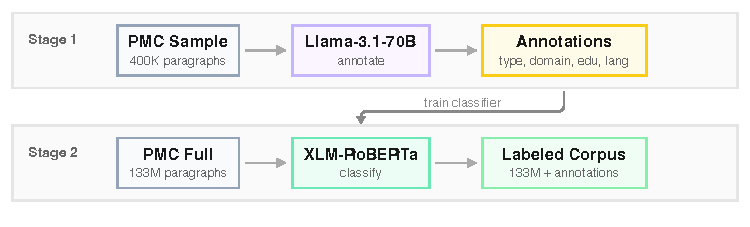
\includegraphics[width=\columnwidth]{sources/part_1/chapter2/imgs/pipeline.pdf}
\caption{\textbf{Two-stage annotation pipeline.} Stage~1: Llama-3.1-70B annotates 0.33\% of PMC paragraphs across four dimensions. Stage~2: a fine-tuned XLM-RoBERTa distills these annotations to label the full corpus, enabling flexible filtering strategies.}
\label{fig:pipeline}
\end{figure}

As \Cref{fig:pipeline} shows, a large model annotates a small fraction of PubMed
Central across four dimensions, and a fine-tuned encoder distills these labels to
the full corpus, which makes paragraph-level filtering possible. Selecting the
relevant paragraphs matches full-corpus pretraining with one third of the tokens,
and its clinical recipe reaches the same point with 2.5 times fewer tokens. The
filter also surfaced about two million clinical cases sitting inside scientific
articles, described in passing and never labelled as clinical text, which were
released as an open set of clinical cases.

Quality is not uniform across the corpus: reviews and studies score highest for
educational value, clinical text varies more, and boilerplate rarely scores well,
which is what makes paragraph-level filtering worthwhile.

Which quality signals actually help is less obvious than it seems. We annotate each
passage with four signals --- educational value, content richness, writing quality,
and terminological precision --- over the 2.16 million annotated passages. Removing
one signal at a time, we find that educational value and content richness improve
performance, while writing quality and terminological precision degrade it. We also
show that generic neural quality filters can amplify benchmark contamination, so a
filter tuned for the general web cannot be trusted on biomedical text without
checking what it selects.
